%The paper size, font size and document type are defined in the following
\documentclass[a4paper,12pt]{article}

%Uncomment the following line, if you write in Finnish (special characters)
%\usepackage[utf8]{inputenc}

%\usepackage[finnish]{babel}
\usepackage[english]{babel}

\usepackage{graphicx}
\usepackage[parfill]{parskip}

%useful special symbols:
\usepackage{amssymb}
\usepackage{latexsym}
\usepackage{amsmath}
\usepackage{amsthm}

\usepackage{listings} % For including code
\usepackage{xcolor}   % For defining code colors


% Define custom colors for the code
\definecolor{codegreen}{rgb}{0,0.6,0}
\definecolor{codegray}{rgb}{0.5,0.5,0.5}
\definecolor{codepurple}{rgb}{0.58,0,0.82}
\definecolor{backcolour}{rgb}{0.95,0.95,0.92}

% Define Python code style
\lstdefinestyle{mystyle}{
    backgroundcolor=\color{backcolour},   
    commentstyle=\color{codegreen},
    keywordstyle=\color{magenta},
    numberstyle=\tiny\color{codegray},
    stringstyle=\color{codepurple},
    basicstyle=\ttfamily\footnotesize,
    breakatwhitespace=false,         
    breaklines=true,                 
    captionpos=b,                    
    keepspaces=true,                 
    numbers=left,                    
    numbersep=5pt,                  
    showspaces=false,                
    showstringspaces=false,
    showtabs=false,                  
    tabsize=4
}

% Apply the style to Python listings
\lstset{style=mystyle}

%a useful package if you write url addresses:
\usepackage{url}
\usepackage{hyperref}

%a package for figures:
% \usepackage[dvips]{color}
% \usepackage{epsfig}

%a package for rotated figures and tables:
\usepackage{rotating}

\usepackage{biblatex}
\addbibresource{references.bib}

\graphicspath{ {./figures/} }

%if you want smaller page margins, uncomment and adjust the following
%\textheight=24.3cm
%\topmargin=-1.8cm
%\textwidth=16.7cm
%\oddsidemargin=-0.3cm
%\evensidemargin=0.0cm


%Create your own environments
\newtheorem{definition}{Definition}
\newtheorem{example}{Example}
\newtheorem{theorem}{Theorem}


\usepackage{placeins}  % Add this line to include the placeins package


%and useful macrosfor faster writing (benefit: you can change the notations 
%later, e.g., two possible notations for your vector x)
\newcommand{\Mmatr}{\ensuremath{\mathbf{M}}}
\newcommand{\xvec}{\ensuremath{\overline{x}}}
\newcommand{\xvecII}{\ensuremath{\mathbf{x}}} %alternative def
\newcommand{\Xset}{\ensuremath{\mathbf{X}}}
\newcommand{\fr}{\ensuremath{\mathit{fr}}} %just neater typing

%If you want to remove the space before paragraphs uncomment the following.
%Remember then to leave an empty line between paragraphs! 
%\setlength{\parindent}{0pt}


\title{MDM-2024 Homework 1}
\author{Cuong Nguyen (101559968), Petteri Raita (909635)\\and Raihan Gafur (101555441)}

%Uncomment the following, if you don't want the date to be printed
%\date{}

\begin{document}

\maketitle
\tableofcontents
\newpage

\listoffigures
\newpage
% Petteri is responsible for 4 and 5

% include tex files of sections here, e.g.
% \input{section1.tex}
% \input{section2.tex}
\section{Methods}
In this experiment, Python was used as the primary programming language, utilizing the
libraries \texttt{numpy} for numerical computations and \texttt{matplotlib} for plotting
and visualization. The randomization interval for generating the data points was the
half-open interval \([0,1[\), excluding the origin. The Lp norms were computed using
a custom function:

\lstinputlisting[language=Python]{code/lp_norm.ipynb}

which supported a range of \(p\) values, including p = 0.5, 0.8, 1, 1.3, 1.5, 1.7, 1.9,
1.95, 2, 5, and \(\infty\). For each experiment, \(q = 100\) data sets, each containing
\(N = 100\) points, were generated across various dimensions \((k = 2, 3, 4, 5, 10, 20,
30, 40, 50, 60, 70, 80, 90, 100, 150, 200, 250, 300)\).

\section{Relative Contrast}
The relative contrast (Ctr) values across various dimensions and Lp norms highlight
the significant impact of dimensionality on the behavior of distance measures. As
observed, the contrast starts very high for small dimensions (e.g., $k=2$) and
decreases as dimensionality increases. For example, for $p=0.5$, the contrast begins
at 27.46 for $k=2$ and gradually converges toward a value around 0.435 when $k=300$,
demonstrating that the differences between the farthest and nearest points diminish
as dimensionality increases. This reduction in contrast aligns with the general
understanding of the curse of dimensionality, where the concentration of distances
in high dimensions makes it harder to distinguish between near and far points. The
trend is similarly observed for other $p$ values, such as $p=1$, $p=2$, and $L_{\infty}$,
though the specific rate of decrease varies.

\begin{figure}
    \centering
    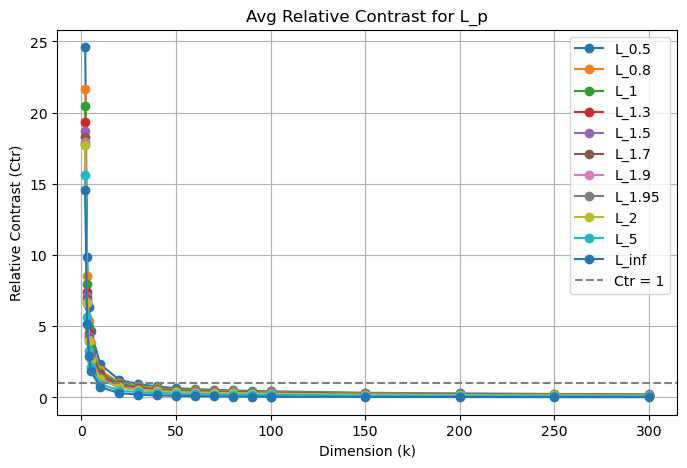
\includegraphics[width=\textwidth, height=\textheight, keepaspectratio]
    {relative-constrast.png}
    \caption{\emph{Avg Relative Contrast} for $L_p$}\label{fig:ctr}
\end{figure}

It can be seen from a closer look of the~\autoref{fig:ctr}, different Lp norms reveals that larger $p$ values tend to produce lower
Ctr values in high-dimensional spaces, indicating that higher norms concentrate distances
more effectively. For instance, in the case of $L_{\infty}$, the Ctr value decreases from
22.29 at $k=2$ to 0.276 at $k=300$, showing a clear convergence trend. Specifically, for
higher $p$ values like $p=2$, the contrast appears to converge around a value of 0.31 as
$k$ approaches 300. Lower $p$ norms, such as $p=0.5$, approach a final contrast value of
approximately 0.435. These values reflect the final state as distances become nearly uniform
at high dimensions. The decrease in contrast across all norms points toward the saturation of
distance values in higher dimensions, where distances become relatively similar. In particular,
the lower $p$ norms like $p=0.5$ show higher initial contrast, reflecting their sensitivity to
small variations, while the convergence rate tends to stabilize more gradually compared to higher
$p$ values. These findings highlight how Lp norms influence the spread of distances in
high-dimensional spaces, with larger $p$ values converging more quickly to a stable contrast value.


% Petteri is responsible for this section
\section{Minimum, Maximum, and Mean Distances}
Present the plots of minimum, maximum and mean distances for each \( L_p \) and discuss the results. How the curves are behaving when \( k \) increases? Can you characterize the form of curves? What is the effect of \( p \)? If a curve seems to be converging, tell also the value that it is approaching.
\subsection{Min-Max-Mean Distance}

P values lower than 1 grow polynomamially.
The following shows the proportionality.

\begin{equation}
    \forall p < 1, \lim_{k \to \infty} \left( \sum_{i=1}^{k} |x_i|^p \right)^{\frac{1}{p}} \propto k^{\frac{1}{p}}
\end{equation}

and p value 1 grows linearly.
\begin{equation}
    \forall p = 1, \lim_{k \to \infty} \left( \sum_{i=1}^{k} |x_i|^p \right)^{\frac{1}{p}} \propto k
\end{equation}

P values greater than 1 grow as p roots of k. The reasoning comes from the norm equation:

\begin{equation}
    \forall p > 1, \lim_{k \to \infty} \left( \sum_{i=1}^{k} |x_i|^p \right)^{\frac{1}{p}} \propto \sqrt[p]{k}
\end{equation}

For all the curves, they can be formulated as curves according to their growth rate, polynomial, linear, or p-root. For the \(\infty\)-norm, the curve can be formulated as a multiplicative inverse curve approaching 1 as k approaches infinity.



All the norms except for \( L_\infty \) diverge as k increases. However, the \( L_\infty \) converges to number one. Mathematically, this follows from the equation for the \( L_\infty \) norm. The values generated are between 0 and 1 and thus the maximum value will be one as k approaches infinity.



\begin{equation}
    \lim_{k \to \infty} \max_{i=1,\ldots,k} |x_i| = 1
\end{equation}



\section{Variance of Distance}
Present the variance plots for each \( L_p \) and discuss the results. How the curves are behaving when \( k \) increases? Can you characterize the form of curves? What is the effect of \( p \)? If a curve seems to be converging, tell also the value that it is approaching.



For all the quasinorms, i.e, norms p < 1. The variance grows polynomially. Since the data is a sample of random datapoints, the sample variance is used.

\[
    \text{Var}(X) = \frac{1}{n -1 } \sum_{i=1}^{n} \left(X_i - \mu \right)^2
\]


\begin{equation}
    \text{Var}_{\text{sample}}\left(\|\mathbf{x}\|_p\right) = \lim_{k \to \infty} \left( \frac{1}{N - 1} \sum_{i=1}^{k} \left( \left( \sum_{i=1}^{k} |x_i|^p \right)^{\frac{1}{p}} - \mathbb{E}\left[\left( \sum_{i=1}^{k} |x_i|^p \right)^{\frac{1}{p}}\right] \right)^2 \right)
\end{equation}

Similar to the min-max-mean distance, the variance grows polynomially for all p < 1. When p = 1, the variance grows linearly. And when p => 2, the variance grows proportionally to a \(\frac{1}{\log(k)}\) function. (or polynomial??).

The interesting case was the norms p between 1 and 2. For those norms, the variance goes to infinity but much slower than for the p=1 linear growth.

All variances larger or equal to 2 converge to 0 as k increases.

In summary, the curves with p < 1 can be characterized as polynomial curves. The curves with $ 1 < p < 2 \propto k^{1/p}$

Should we add images??

\section{Extra Experiments}
Further experiments were conducted with an increased dimensionality, specifically within
the range of $100 < k <= 300$. The results indicate a consistent trend, with no discernible
turning point. The patterns previously reported continue to persist and, if applicable,
move towards a convergence point.

Furthermore, a series of $p$ values within the range of $0.5 < p < 2$ were examined,
focusing on the \emph{Avg} statistics values. Notably, the \emph{Avg Variance} revealed
novel insights, as detailed in~\autoref{sec:variance}. A distinct pattern shift
was observed in the \emph{Avg Variance} corresponding to $p={1,2}$, transitioning from
an increasing trend to a decreasing one. Upon investigating intermediate $p$ values
(1.7, 1.9, and 1.95), it was discovered that the transition point may initiate at $p=1.95$.
This is where the \emph{Avg Variance} pattern begins to slightly decrease as the dimensionality,
denoted by $k$, increases.

\begin{figure}[ht!]
    \centering
    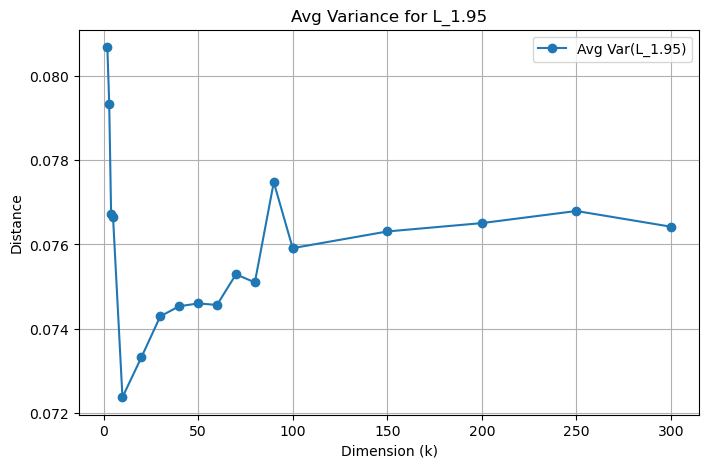
\includegraphics[width=0.8\textwidth,height=\textheight]
    {lp-turning-point.png}
    \caption{\emph{Avg Variance} for $L_{1.95}$}\label{fig:lp-turning-point}
\end{figure}

\section{Conclusion}
Upon examination of the statistical properties, including \emph{min}, \emph{max},
\emph{mean}, \emph{variance}, and \emph{relative contrast}, it can be inferred
that the ``curse of dimensionality'' gives rise to unanticipated behaviors within
high-dimensional spaces. Specifically, the growth in dimensionality can yield
the following consequences:


\begin{itemize}
    \item Convergence of \emph{min}, \emph{mean}, and \emph{max} distances,
    causing the majority of data points to become equidistant.
    \item Decrease in \emph{variance} of distances, making distances of data
    points approach zero.
    \item Approach of \emph{relative contrast} towards zero, thereby
    diminishing the distinction between proximate and distant points.
\end{itemize}

In light of these observations, it becomes evident that the "curse of
dimensionality" poses significant challenges for certain machine learning
algorithms when operating in high-dimensional settings, thus necessitating 
appropriate adjustments to ensure optimal performance.

%Bibliography style. The alpha style generates references with 
%first letters and year. If you prefer numbers, use style plain.
% \bibliographystyle{alpha}
% \bibliographystyle{plain}
% \bibliography{ref}

\printbibliography{}

% Appendices
\begin{appendix}
  All code is publicly available on GitHub at \url{https://github.com/ancuongnguyen07/CS-E4650/tree/master/hw5}
\end{appendix}


\end{document}
